\chapter{Definición del problema}\label{cap:trabajo_relacionado}


\section{Redes neuronales convolucionales}
Las redes neuronales convolucionales CNN por sus siglas en ingles, es un tipo de modelo de aprendizaje profundo para procesar datos que tiene un formato de cuadrícula, como las imágenes. Está inspirado en la organización de la corteza visual de los animales, diseñada para aprender de forma automática y adaptativa, patrones en jerarquías, de bajo a alto nivel. Por lo genera una red CNN se compone de tres tipos de capas: convolución, agrupación y capas completamente conectadas, como se puede ver en \autoref{fig:CNNEjemplo}. Las dos primeras, realizan extracción de características, mientras que la tercera, las relaciona  y genera una salida. La capa de convolución desempeña un papel clave en CNN, se compone de una pila de operaciones matemáticas, como la convolución, que es un tipo especializado de operación lineal. En las imágenes en 2D estas redes son muy utilizadas, por su alta eficiencia para tareas de visión artificial, como en la clasificación y segmentación de imágenes, entre otras aplicaciones.\\

Algunos ejemplos de redes CNN son, VGG16 que posee 13 capas de convolución, 5 de agrupación y una totalmente conectada. AlexNet conocida por ganar la competencia 2012 ImageNet LSVRC-2012, contiene 5 capas convolucionales, 3 capas de agrupación y 3 capas completamente conectadas.\\

Las redes CNN se a utilizado para resolver distintos problemas como, la detección de objetos, Fast R-CNN \cite{girshick2015fast}. La comprensión visual de escenas de calles urbanas \cite{cordts2016cityscapes}, entre otros.
En este trabajo utilizamos la salida de las redes CNN (la capa completamente conectada), como un vector de características visual de la imagen. Debido a que son muy eficaces reconociendo patrones, los vectores de dos imágenes que tienen un aspecto similar, también tienden a tener una semejanza. 

\begin{figure}
	\centering
	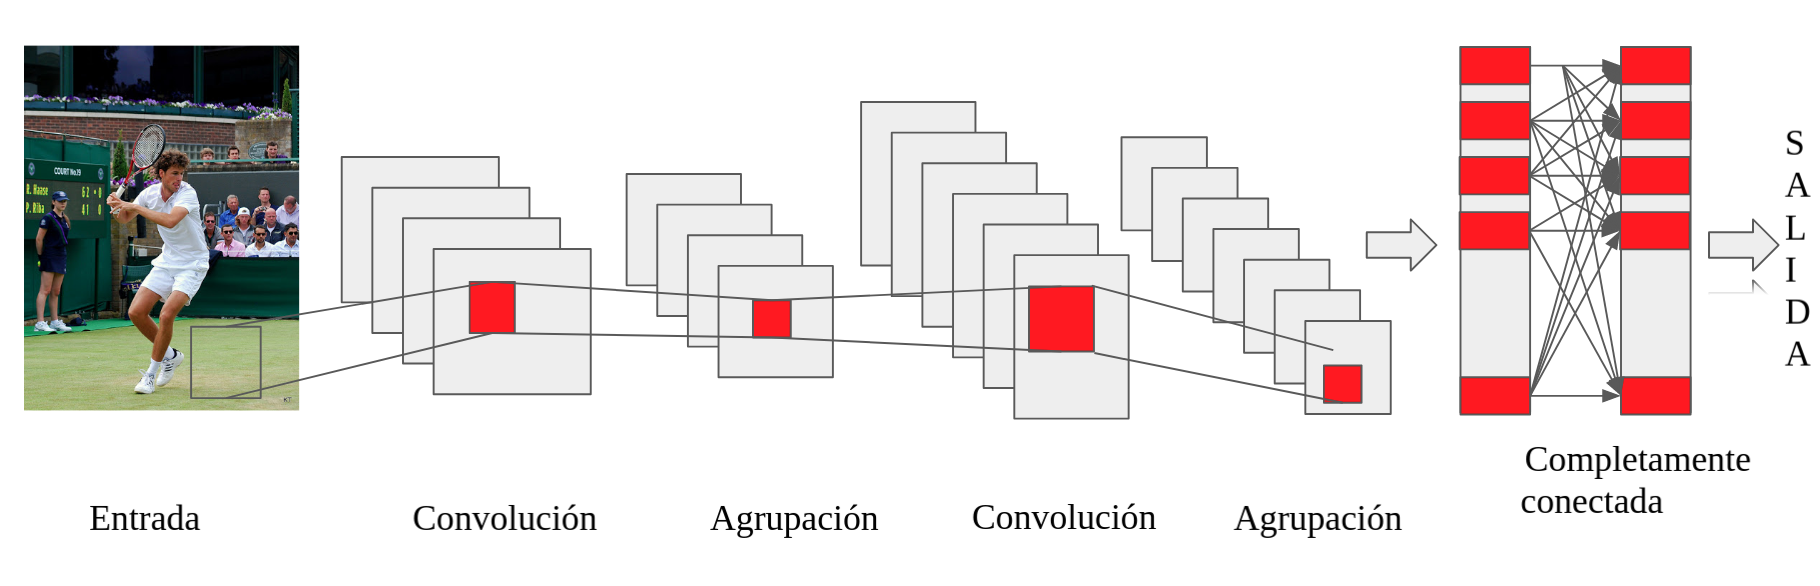
\includegraphics[width=0.9\textwidth]{img/red_cnn.png}
	\caption{Una arquitectura simplificada de una rede neuronal convolucional.}
	\label{fig:CNNEjemplo}
\end{figure}

\section{Word embedding}
Al igual que con las imágenes, que utilizamos las redes CNN, para obtener un vector que represente a la misma, es necesario un procedimiento para poder representar las palabras, con algún objeto matemático. Hay muchas formas de representar palabras, pero la mas conocida es word embedding, es una técnica de aprendizaje en el campo de procesamiento del lenguaje natural (PLN). Es capas de capturar el contexto de una palabra en un documento, calcular similitud semántica y sintáctica con otras palabras, etc.\\

Para entender como funcionan, consideremos las oraciones con un significado similar: ``Que tengas un buen día.'' y ``Que tengas un gran día.''. Si construimos un vocabulario exhaustivo 
 \[ V = \{que, tengas, un, buen, gran, dia\}. \]
 Ahora, si creemos un vector codificado para cada una de estas palabras. En donde cada vector tiene el tamaño de V y son todos 0 excepto por el elemento en el índice que representa la palabra correspondiente en el vocabulario, que contiene un 1. No resulta una buena representación ya que la distancia entre \textit{gran} y \textit{buen} es la misma que entre \textit{tengas} y \textit{buen}.  El objetivo es que las palabras con un contexto similar ocupen posiciones espaciales cercanas. Para lograr esto, se introduce cierta dependencia de una palabra de las otras.\\

Word2Vec \cite{mikolov2013distributed} desarrollado por Tomas Mikolov en 2013. Es un modelo particularmente eficiente desde el punto de vista computacional. Este modelo se encuentra disponible de dos formas: Continuous Bag-of-Words (CBOW) o el modelo Skip-Gram. En CBOW, las representaciones distribuidas de contexto (o palabras circundantes) se combinan para predecir la palabra en el medio. En nuestro ejemplo \textit{gran} y \textit{buen} están rodeado de un contexto similar por lo cual resultan en vectores similares. Es varias veces más rápido de entrenar que el skip-gram, y tiene una precisión ligeramente mejor para las palabras frecuentes. Mientras que en el modelo Skip-gram, la representación distribuida de la palabra de entrada se usa para predecir el contexto. Se entrena con una tarea falsa que, dada una palabra, intentaremos predecir las palabras vecinas. En realidad, el objetivo es solo aprender los pesos de la capa oculta que son en realidad los ``vectores de palabras'' que estamos tratando de aprender. \textit{Gran} se entrena para predecir el contexto \textit{un} y  \textit{dia}, al igual que con \textit{buen}. Funciona bien con una pequeña cantidad de datos de entrenamiento, representa bien incluso palabras o frases raras.

En este trabajo, aprovechamos la capacidad de capturar similitudes semántica que tiene word embedding, para relacionar las clases vistas con las clases no vistas. Utilizamos un modelo pre-entrenado generado a partir de word2vec para representar las palabras de las distintas clases.\\


\section{Propuestas de objetos}
En problemas de detección de objetos, generalmente se tiene que encontrar todos los objetos posibles en la imagen, como todos los autos todas las bicicletas, etc. La localización de objetos se refiere a identificar la ubicación de uno o varios objetos en la imagen. Un algoritmo de localización de objetos generará las coordenadas de la ubicación de los objetos con respecto a la imagen. En visión artificial, la forma más popular de representar la ubicación de los objetos es con la ayuda de cuadros delimitadores (Bounding Boxs). Existen muchos algoritmos y redes que intenta resolver este problema como por ejemplo, \textbf{ventana deslizante}, \textbf{Edge-Boxes} \cite{zitnick2014edge}, \textbf{Selective search} \cite{uijlings2013selective} ect. En ZSD las propuestas de objetos cumple un papel importante, ya que se necesita extraer todas las instancias de los objetos, pero también tiene que discriminar fondos como cielo, fondo de ciudad, veredas, ect. Es muy difícil encontrar un equilibrio ya que un algoritmo poco ``permisivo'' ignorara muchas instancias de objetos y por el otro extremo, se incluirá fondos y de esta manera introducir ruido en nuestro modelo.\\

En este proyecto, como veremos en el \autoref{cap:experimentos} se probo con \textbf{Edge-Boxes} y \textbf{Selective search}, ya que estas generan una cantidad significativamente menor a algoritmos del estilo de ventana deslizante. Aun asi, procesar todas estas propuestas es engorroso. Ademas, estos modelos por lo general dan como resultados muchos cuadros con una gran superposición. Esto da lugar a una técnica denominada Supresión no máxima (NMS) \ref{fig:NMS}. Este algoritmo necesita de un puntaje que indica la confianza del cuadro delimitador y un criterio para comparar entre distintos cuadros. El criterio mas común es Intersección sobre Unión (IoU), en la imagen ~\ref{fig:IoU} se muestra como se calcula sobre dos Bounding Boxs. La salida de NMS es un conjunto mas reducido de propuestas, en la cual se filtraron todas las que se consideran repetidas y retorna solo las mas representativa. A continuación se muestra el pseudocódigo de NMS.

\begin{center}
\noindent\fbox{
	\begin{minipage}{1\textwidth}
		\begin{algorithmic}[1]
			\Procedure{NMS}{B, S, t}
				\State{D = $\emptyset$ }
				\For {B $\neq \emptyset$ }
					\State{$b_i$ = \textbf{SelPropuestaMaxPuntaje}(B, S)}
					\State{\textbf{Eliminar}($b_i$, B)}
					\For {$b_j$ $\in$ B}
						\If {\textbf{IOU}($b_i$, $b_j$) $>$ t}
							\State{\textbf{Eliminar}($b_j$, B)}
						\EndIf
					\EndFor				
				\EndFor
			\State{\Return {D}}
			\EndProcedure
		\end{algorithmic}
	\end{minipage}
}
\end{center}
\begin{figure}[]
	\begin{subfigure}{.4\textwidth}
		\centering
		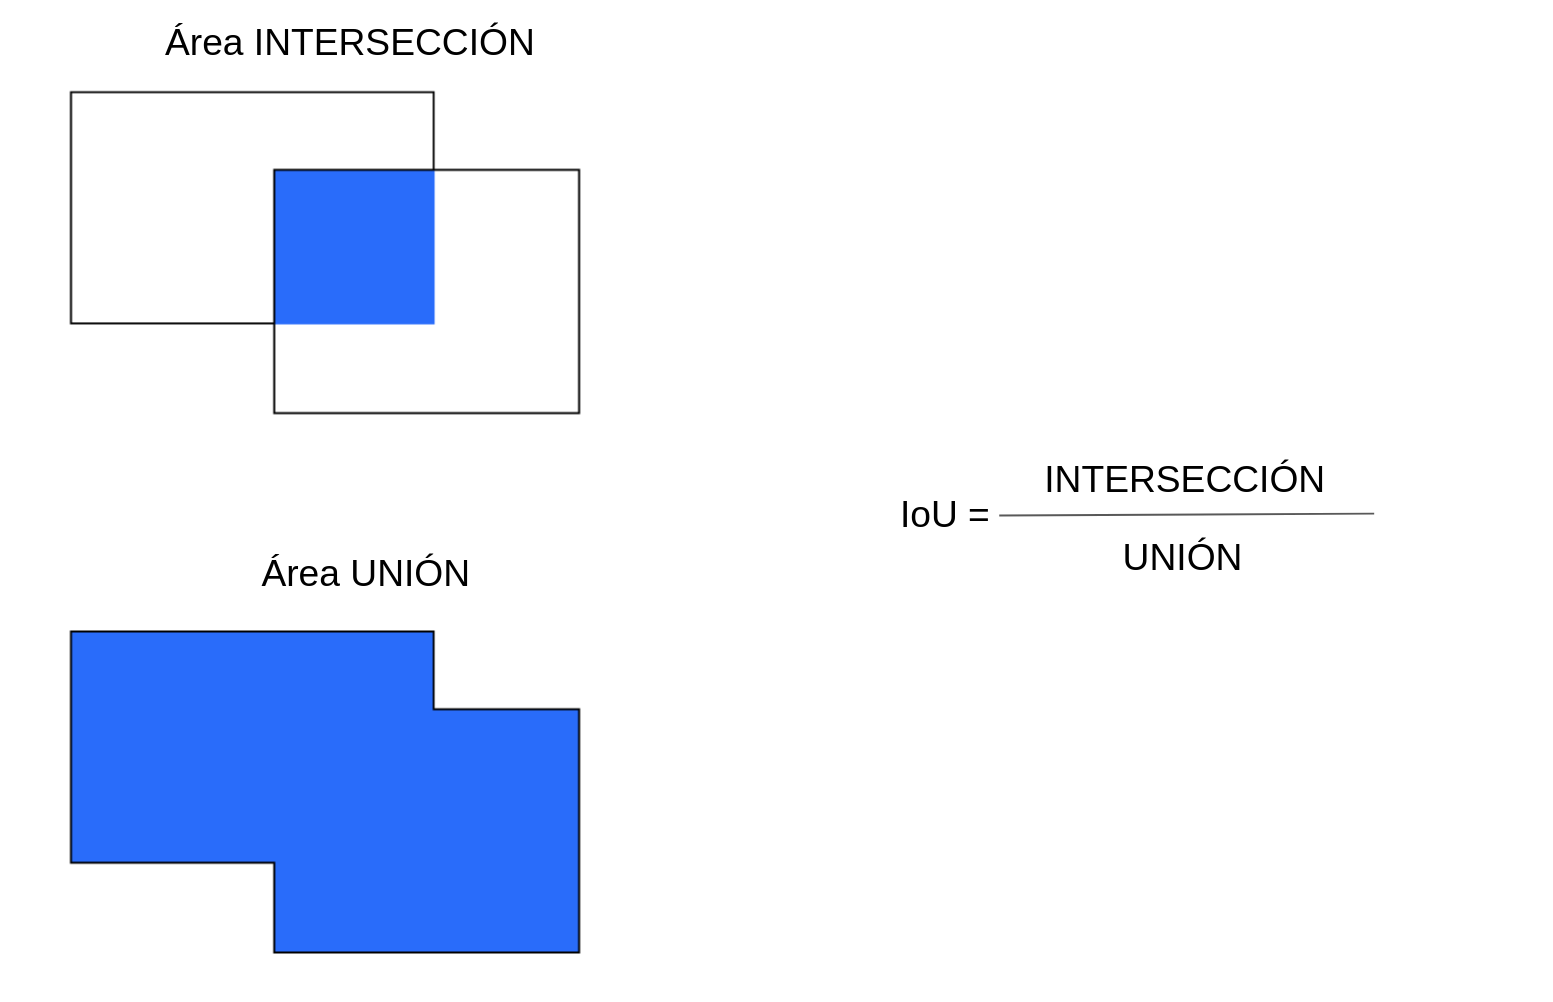
\includegraphics[width=0.7\textwidth]{img/iou.png}
		\caption{Iou}
		\label{fig:IoU}
	\end{subfigure}
	\begin{subfigure}{.6\textwidth}
		\centering
		\centering
		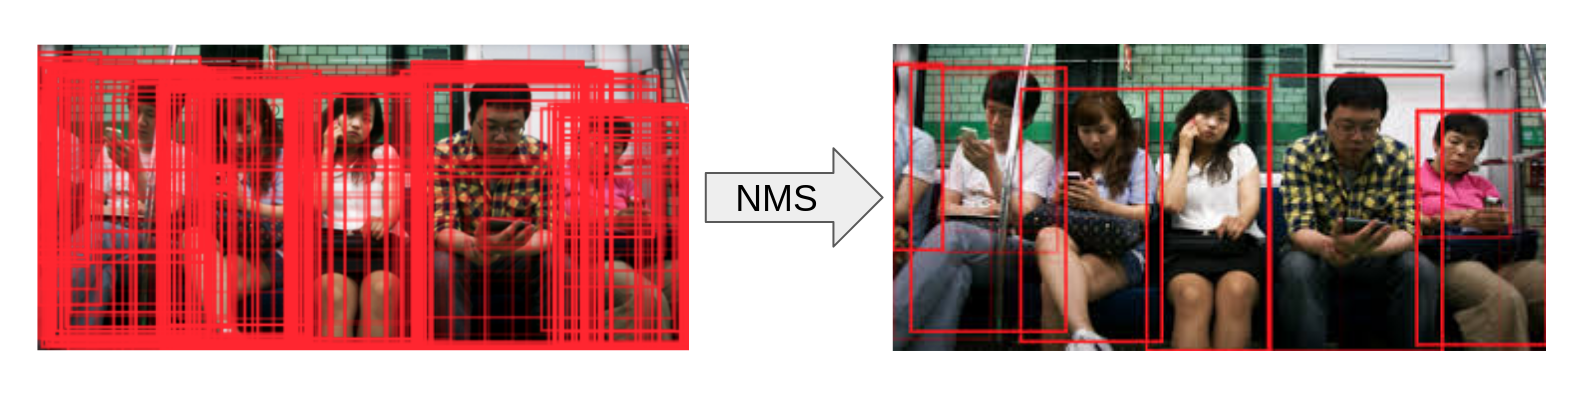
\includegraphics[width=1.1\textwidth]{img/NMS.png}
		\caption{Supresión no máxima}
		\label{fig:NMS}
	\end{subfigure}
	\caption{(a) Calculo de Intersección sobre Unión. (b) Salida de la propuesta de objetos y el resultado después de NMS.}
		\label{fig:RP}
\end{figure}

\section{Multimodales}

Nuestra experiencia del mundo es multimodal, vemos objetos y sus entornos, escuchamos música y ruidos, sentimos la textura de los distintos materiales, olemos los aromas que no rodean y probamos el sabor de un buen plato de comida.  Inconscientemente asociamos una situación a los distintos estímulos que recibimos en ese momento y los relacionamos entre si, para genera una idea de lo que esta sucediendo. De esta manera, sabemos que si algo huele mal lo mas probable que sepa igual y podemos relacionar una imagen del campo con el sonido de los pájaros.\\

La modalidad se refiere a la forma en que algo sucede o se experimenta. Un problema de investigación se caracteriza como multimodal cuando incluye datos de distinta naturaleza. Para que la inteligencia artificial avance en la comprensión del mundo que nos rodea, necesita poder interpretar y relacionar estas distintas señales. Aunque la combinación de diferentes modalidades para mejorar el rendimiento parece una tarea intuitivamente atractiva, en la práctica, es un desafío, y una ineducada combinación de distintos tipos de información, puede generar ruido y conflictos. La idea general es, partir de dos objetos matemáticos distintos uno de cada modal y poder transformar a ambos para lograr que pertenezcan a un tercer objeto que es la representación multimodal. Las imágenes suelen estar asociadas con etiquetas y explicaciones de texto. En este trabajo nos aprovechamos esto y tratamos de encontrar un espacio común entre el vector que representan a la imagen del objeto y el que representa la sintaxis del mismo.


\section {Aprendizaje por disparo cero (ZSL)}
Es un conjunto de problemas de aprendizaje automático, donde en el momento de la prueba, se observan muestras de clases que no se observaron durante el entrenamiento y se necesita predecir la categoría a la que pertenecen. A diferencia de las configuraciones estándares en el aprendizaje automático, donde se espera que se clasifiquen correctamente las nuevas muestras en las clases que ya han observado durante el entrenamiento, en ZSL, no se han proporcionado muestras de las clases durante el entrenamiento del clasificador. Podemos diferenciar dos tipos de clases, las vitas que están presente en el entrenamiento y las invisibles o novedosas que no estuvieron. Naturalmente, se debe proporcionar algún tipo de información complementaria sobre estas clases invisibles, este tipo de dato puede ser variado. Una descripción estructurada predefinida, que al tenerla en cuenta mejora el aprendizaje. Una descripción textual, aquí las clases van acompañadas de un comentario en lenguaje natural. Esto podría incluir, por ejemplo, una descripción de wikipedia. Por ultimo, tanto las clases visibles como las invisibles están relacionadas en un espacio vectorial, donde el conocimiento de las clases vistas se puede transferir a clases invisibles.\\

El problema de aprendizaje por disparo cero se puede dividir en categorías según los datos presentes durante la fase de entrenamiento y la fase de prueba.\\
\textbf{Con base en los datos disponibles en el momento de entrenar un modelo}
\begin{itemize}
	\item \textbf{Aprendizaje por disparo cero inductivo:} Se tiene acceso a datos de imágenes etiquetadas de las clases vistas.
	\item \textbf{Aprendizaje por disparo cero transductivo:} Además de los datos de imagen etiquetados de las clases vistas, también se tiene acceso a las imágenes no etiquetadas de las clases no vistas.
\end{itemize}
\textbf{Basado en los datos disponibles en el momento de la inferencia}
\begin{itemize}
	\item \textbf{Aprendizaje por disparo cero convencional (ZSL):} En las pruebas solo se evalúan las clases no vistas.
	\item \textbf{Aprendizaje por disparo cero generalizado (GZSL):} En las pruebas se evalúan tanto las clases vista como las no vistas.
\end{itemize}


\section {Detección de objeto por disparo cero (ZSD)}\label{cap:ZSD}
La Detección de objeto por disparo cero (ZSD), tiene como objetivo reconocer y localizar simultáneamente instancias de objetos que pertenecen a categorías novedosas sin ningún ejemplo de entrenamiento. Como estas categorías no están presente en entrenamiento resulta imposible, tener alguna información sobre su aspecto visual, lo cual no nos permite detectarlas ni reconocerlas. Es necesario encontrar algún dominio que tenga la capacidad de guardar la información de todas las clases, para luego relacionarlas con el aspecto visual de las categorías novedosas. \\

En este trabajo, proponemos un modelo de disparo cero inductivo, es decir, solo observamos imágenes de clases vistas y etiquetas que indican a que clase pertenece. Estas etiquetas son palabras del lenguaje natural sin ninguna estructura. Luego se puede inferir todas las clases o solo las invisibles, dependiendo de lo que se quiere evaluar, aprendizaje por disparo cero generalizado o convencional.\\ 


Para formalizar, denotamos las clases como $\mathcal{C} = \mathcal{S} \cup \mathcal{U}$, donde $\mathcal{S}$ son las clases vistas para entrenamiento y $\mathcal{U}$ las clases no vistas, utilizadas en la etapa de pruebas. Ademas se tiene que $\mathcal{S} \cap \mathcal{U} = \emptyset$. Aunque no es necesario definir el conjunto de clases de pruebas, ya que el modelo tiene que ser capas de detectar tanto clases vista como las no vista, se hace para poder tener una evaluación cuantitativa.\\
Denotamos a una imagen como $\mathcal{I} \in \mathbb{D}^{\mathcal{M} \times \mathcal{N} \times 3}$. Donde $\mathbb{D} = \{0,...,255\}$, $\mathcal{M}$  es el largo de la imagen, $\mathcal{N}$ el ancho. Esta es la forma en la que se representa cada pixel de la imagen en el formato \textbf{RGB}, donde se tiene 3 canales que caracterizan la intensidad de los colores rojo, verde y azul. Por cada imagen se provee un conjunto de cuadros delimitadores  $\mathbb{B} = \{b_0,...,b_k\mid b_i \in N^4\}$ y sus etiquetas asociadas como $\mathbb{Y} = \{y_0,...,y_k\mid y_i \in \mathcal{C}\}$. Para cada cuadro delimitador $b_i$ extraemos una característica profunda utilizando una red neuronal convolucional denotada como $\phi(b_i) \in \mathbb{R}^{D_1}$. Denotamos las incrustaciones semánticas $w_j \in  \mathbb{R}^{D_2}$ obtenido por algún modelo de \textbf{Word embedding} para cada etiqueta $y_i$. El conjunto de todas las imágenes de entrenamiento se indica con $\mathcal{X}^s$, que contiene ejemplos de todas las clases de objetos visibles.  El conjunto de todas las imágenes de prueba que contienen muestras de clases de objetos invisibles se indica con  $\mathcal{X}^u$. En particular, no hay ningún objeto de clase invisible en $\mathcal{X}^s$, pero $\mathcal{X}^u$ puede contener objetos vistos.

El objetivo es encontrar una matriz de proyección $W_p$, tal que \[ \psi_i = W_p\phi(b_i) \:\:\:\mid\:\:\: W_P \in \mathbb{R}^{D_2 \times D_1},\:\:\: \psi_i \in \mathbb{R}^{D_2} \] Notar que $\psi_i$ y las incrustaciones semánticas se encuentran en el mismo dominio. Como mencionamos en secciones anteriores, el espacio vectorial semantico, tiene una gran capacidad de capturar similitudes semántica. Por lo cual resulta clave encontrar una matriz que para cada cuadro delimitador se proyecte lo mas cerca posible a la incrustación semántica de su clase. En otras palabras se quiere una función $f : \mathcal{X} \to \{y_0,...,y_k\mid y_i \in \mathcal{C}\}$ con $\mathcal{X} =  \mathcal{X}^s \cup \mathcal{X}^u$ que da el riesgo empírico regularizado mínimo $\mathcal{R}$ de la siguiente manera: \[ \arg_{}\min_{f \in F} \mathcal{R}(f(x,W_p)) \] donde, $x \in \mathcal{X}^s$ durante el entrenamiento. La función de mapeo utilizado en las pruebas, tiene la siguiente forma \[ f(x,W_p) = \arg_{}\max_{y \in \mathcal{C}}\max_{b \in \mathbb{B}(x)} (F(x,y,b,W_p))\] donde $\mathbb{B}(x)$ son las propuestas de la imagen $x$. Intuitivamente, se busca los cuadros delimitadores de mejor puntuación y se les asigna la categoría de objeto de puntuación máxima.\\

El estricto requisito de no utilizar ninguna imagen de clase invisible durante el entrenamiento en si mismo es una condición difícil. Pero existen otras dificultades de la tarea de detección de disparo cero que están asociado al conjunto de datos de entrenamiento y prueba, es decir entre las clases vistas e invisibles, que lo dificultan mas.


\begin{itemize}
	\item \textbf{Rareza}: los conjuntos de datos por lo general, contiene un problema de distribución, es decir, muchas clases raras obtienen menos cantidad de instancias. Este problema hace que las clases con mayor cantidad de instancias sesguen el modelo y en las pruebas las clases mas raras y las relacionadas a ella sean marcadas incorrectamente. Es evidente que una clase invisible debería estar dentro del conjunto de clases raras, pero esto implica introducir información extra que en la vida real no es posible. Esto es un problema al tiempo de comparar dos modelos que fueron entrenados con distintas clases ya que algunas separaciones resultan mejores que otras.

	\item \textbf{Tamaño del objeto}: algunas clases de objetos raros como tijeras, lapicera, celulares, etc., suelen tener un tamaño pequeño. Los objetos más pequeños son difíciles de detectar y reconocer. También, tienen el problema que por lo general están juntos a objetos mas grandes como una mesa o persona y se ven opacadas por estas clases.

	\item \textbf{Alta diversidad}: cada clase pertenece a un conjunto donde se encuentran todas las clases similares o que tienen alguna relación, que llamaremos metaclase. Cada metaclase recibe un número diferente de clases y existe una gran diversidad visual en las imágenes de cada metaclase o clase superior. Dado que estar en una misma metaclase no garantiza la similitud visual, es difícil aprender relaciones para las categorías invisibles que son bastante diferentes de las categorías vistas en la misma metaclase. Por ejemplo, ``auto'' tiene muchas clases similares en comparación con ``cartel''. Esto permite una descripción inadecuada de la clase invisible que eventualmente afectará el rendimiento de detección de disparo cero.

	\item \textbf{ Ruido en el espacio semántico}: cuando se utiliza los vectores de incrustación semántica no supervisados como word2vec o GloVe. Las incrustaciones resultante  en general son ruidosas, ya que se generan automáticamente a partir de la minería de texto no anotado. Esto también afecta significativamente el rendimiento de la detección de disparo cero.
\end{itemize}


Existen algunas variaciones del problema de ZSD, que intentan aliviar estos problemas, siendo un poco mas permisivos. Como \textbf{Detección de metaclase de disparo cero (ZSMD)}, que dada una imagen de prueba, el objetivo es localizar cada instancia de una clase de objeto invisible y categorizarla en una de las superclases. \textbf{Etiquetado de disparo cero (ZST)}, para reconocer una o más clases invisibles en una imagen de prueba, sin identificar su ubicación. \textbf{Etiquetado de metaclase de disparo cero (ZSMT)}, para reconocer una o más metaclases en una imagen de prueba, sin identificar su ubicación. Pero estas tareas son buenas para calcular resultados cuantitativos y no para ser utilizados en problemas reales.
